\vspace{10.0cm}}
\section{Análise de Desempenho  Experimental\label{section:context}}
% What is the problem being worked on?
% What was the state-of-the-art before the paper was written?
% What impact did the paper have (if known)? 

\justifying
\noindent
\subsubsection{Integer Score e Floating Point Score }
\centerline{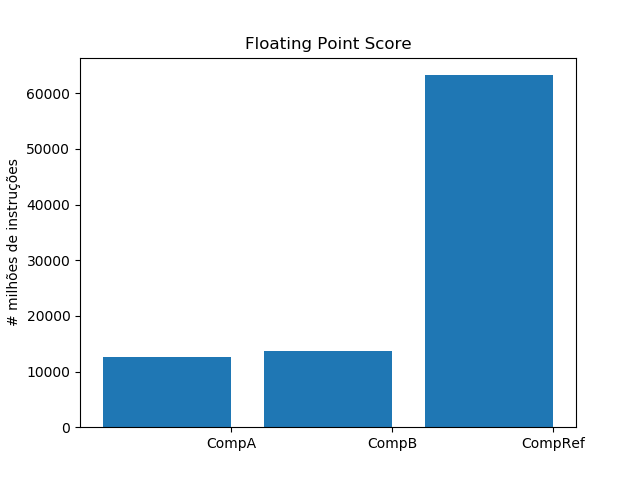
\includegraphics[width=120mm]{images/1.png}}
\centerline{Figura 1: Gráfico referente a Floating Point Score}}
\vspace{1.5 cm}} 

\centerline{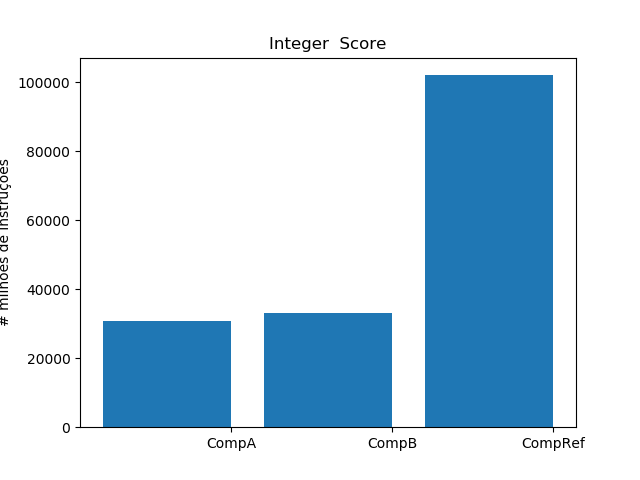
\includegraphics[width=120mm]{images/2.png}}
\centerline{Figura 2: Gráfico referente a Integer Score}}
\vspace{0.5cm}
Percebe-se que o computador de referência tem um valor maior de MIPS e MFLOPS que os demais computadores, além disso, pode-se ressaltar que o computador de referência tem o clock maior que o computador A e o tempo de execução menor que o computador A e B.
\vspace{1.5 cm}} 

\subsubsection{Latência x  Tipo de memória}

\centerline{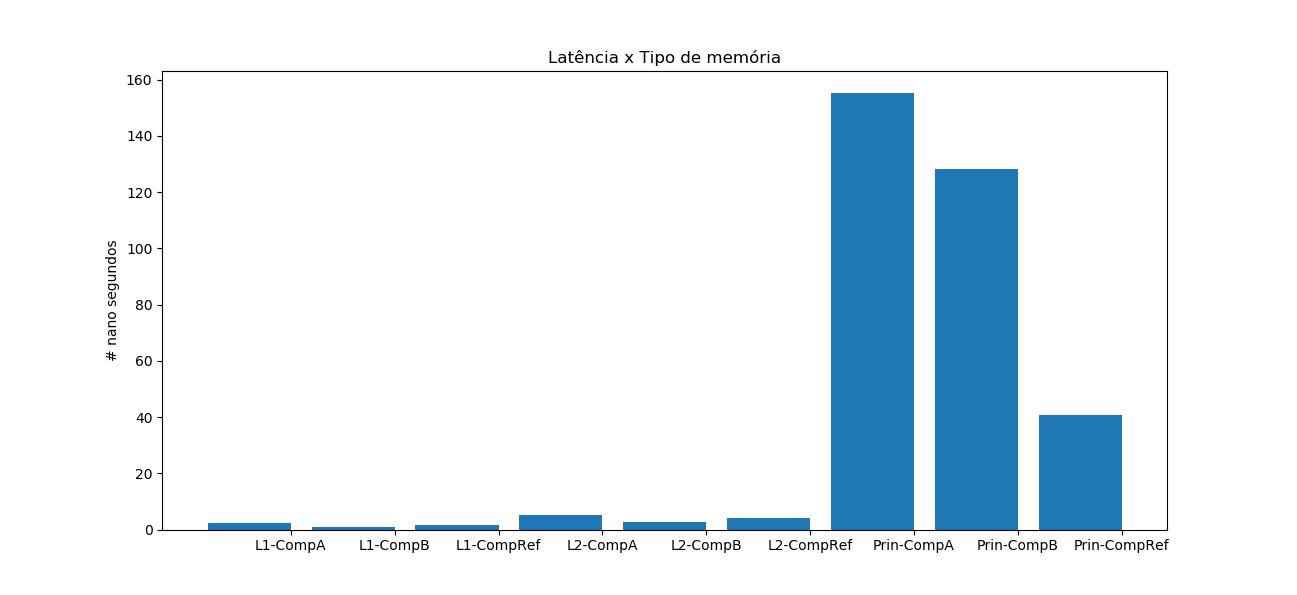
\includegraphics[width=200mm]{images/3.png}}
\centerline{Figura 3: Gráfico referente a Latência x  Tipo de memória}}
\vspace{1.5 cm}} 
É possível inferir a partir do gráfico acima que, o Computador de Referência obteve melhor desempenho seja na memória L1,L2 ou Primária.
%-------------------------------------------------------------------

\end{text}